\documentclass[times, utf8, zavrsni]{fer}
\usepackage{booktabs}
\usepackage{subfig}
\usepackage{algorithm}
\usepackage{algpseudocode}
\begin{document}

% TODO: Navedite broj rada.
\thesisnumber{3948}

% TODO: Navedite naslov rada.
\title{Raspoznavanje objekata konvolucijskim neuronskim mrežama}

% TODO: Navedite vaše ime i prezime.
\author{Dario Smolčić}

\maketitle

% Ispis stranice s napomenom o umetanju izvornika rada. Uklonite naredbu \izvornik ako želite izbaciti tu stranicu.
\izvornik

% Dodavanje zahvale ili prazne stranice. Ako ne želite dodati zahvalu, naredbu ostavite radi prazne stranice.
\zahvala{}

\tableofcontents

\chapter{Uvod}
Računalni vid je područje koje uključuje metode za dohvaćanje, obrađivanje i shvaćanje slika i općenito podataka velikih dimenzija te je zanimljivo područje računalne znanosti zbog mogućnosti široke primjene u današnjem svijetu. Jedna od podgrana ovog područja je raspoznavanje objekata.

Ljudi su sposobni prepoznati mnoštvo različitih objekata sa jako malo truda no za računala je to složen proces koji ima brojna ograničenja koja ljudi nemaju. Uzmimo u obzir da se slika u računalu reprezentira kao višedimenzionalni niz jačina svjetlosti. Promjene u prikazu objekta poput različite orijentacije, skaliranja, i osvijetljenja objekta su u digitalnim slikama prestavljene sa različitim podatcima. Objekt također može biti i zaklonjen. Dobar model raspoznavanja mora biti otporan na ove varijacije te je zato problem raspoznavanja objekata još uvijek neriješen i u zadnjih nekoliko desetljeća su razvijene brojne metode kojima se pokušava riješiti ovaj problem.
Za razliku od pisanja klasičnih algoritama poput sortiranja brojeva za problem klasifikacije objekata nije očito kako bi se mogao napisati takav algoritam gdje su sve varijacije ulaza posebno obrađene u kodu. Zato se za klasifikaciju objekata koristi pristup usmjeren na podatke (engl. \textit{data-driven approach}). Programu se da veliki broj ulaza sa velikom količinom primjera za svaku klasu te se razvije algoritam učenja koji učitava date primjere te uči o vizualnom prikazu svake klase. Takve programe nazivamo klasifikatorima.

U zadnjih nekoliko desetljeća su razvijeni različiti klasifikatori za što točnije prepoznavanje objekata. Među tim klasifikatorima su i umjetne neuronske mreže. Ispostavilo se da se sa dubokim neuronskim mrežama trenutno dobivaju najbolji rezultati za problem klasifikacije. Najkorišteniji oblik dubokih neuronskih mreža u račnunalnom vidu su konvolucijske neuronske mreže.

Cilj ovog rada je razviti implementaciju konvolucijske neuronske mreže za primjenu na osobnim računalima, optimirati hiperparametre mreže te vrednovati učinak naučene mreže. Razvijena mreža će se testirati na skupu MNIST rukom pisanih znamenki.
\chapter{Neuronske mreže}
Područje umjetnih neuronskih mreža (engl. \textit{Artificial Neural Networks - ANN}) je prvotno bilo inspirirano sa modeliranjem biološkog živčanog sustava, a tek kasnije se počelo koristiti u sklopu strojnog učenja. 
\section{Neuron}
Radi razumijevanja neuronske mreže potrebno je prvo razumijeti funkcioniranje jednog neurona. Ljudski živčani sustav se sastoji od otprilike 86 bilijona neurona koji su povezani sa $10^{14}$ do $10^{15}$ sinapsi. Svaki neuron dobiva svoje ulazne signale kroz dendrite i šalje izlazni signal kroz akson. Akson je sa sinapsama spojen sa dendritima drugih neurona. Na slici ~\ref{fig:bio-neuron} možemo vidjeti izgled biloškog neurona.
\begin{figure}
    \centering
    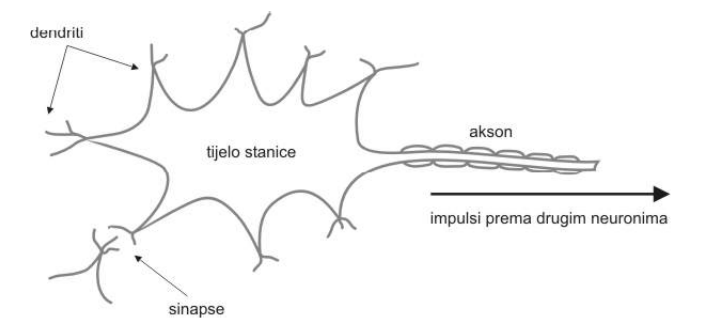
\includegraphics[width=12cm]{img/bio-neuron.png}
    \caption{Biološki neuron}
    \label{fig:bio-neuron}
\end{figure}

U modelu umjetnog neurona signali koji putuju aksonom (npr. \textbf{$x_{0}$}) se množe sa sinaptičkim snagama dendrita(težinama) drugih neurona (npr. \textbf{$w_{0}$}). Ideja je da se sinaptičke snage mogu mijenjati sa učenjem te određuju utjecaj jednog neurona na drugi. Svaki neuron ima aktivacijsku funkciju koja uzima sumu umnoška ulaza neurona sa pripadnim težinama i praga ($\theta$) te ih preslikava na izlaz neurona koji modelira signal na aksonu($y$). Na slici ~\ref{fig:umj-neuron} možemo vidjeti model umjetnog neurona. 
\begin{figure}
    \centering
    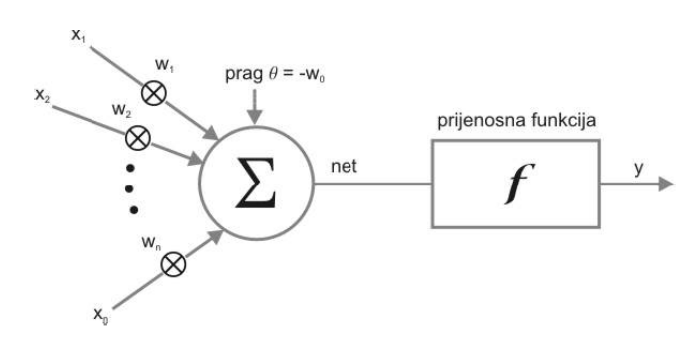
\includegraphics[width=12cm]{img/umj-neuron.png}
    \caption{Umjetni neuron}
    \label{fig:umj-neuron}
\end{figure}

Označimo ulaze sa $x_{1},x_{2},...,x_{n}$ te njihove pripadne težine sa $w_{1},w_{2},...,w_{n}$, i prag sa $\theta$. Onda možemo izlaz neurona zapisati kao:
\begin{equation}
y = f(\displaystyle\sum_{i=1}^{n}(x_i*w_i) + \theta)
\end{equation}
Radi pojednostavljenja se često uzima oznaka $w_0$ umjesto $\theta$ te se dodaje jedan ulaz $x_0$ koji je stalno jednak 1. Sa ovom modifikacijom izlaz se može izraziti kao:
\begin{equation}
y = f(\displaystyle\sum_{i=0}^{n}(x_i*w_i))
\end{equation}
\subsection{Aktivacijske funkcije}
Postoje veliki izbor aktivacijskih funkcija no u praksi se koriste samo neke koje su se pokazale korisnima. Spomenuti ćemo četiri različite aktivacijske funkcije (slika ~\ref{fig:aktivacijske-funkcije}) te njihove karakteristike.

Najobičnija aktivacijska funkcija je linearna aktivacijska funkcija koja je preslikava svoj ulaz na izlaz. Ovakav tip aktivacijske funkcije ne koristimo u dubokim neuronskim mrežama zato što onemogućava učenje mreže. 

Step funkcije u neuronima funkcioniraju kao prekidači. Izlaz funkcije može poprimiti samo dvije različite vrijednosti ovisno o tome da li je ulaz manji ili veći od nekog praga. Primjer jedne ovakve funkcije je:
\begin{equation}
  f(x) = \begin{cases}
    0, & \text{$x<0$}\\
    1, & \text{$x\geq0$}
  \end{cases}
\end{equation}
Ovakva funkcija je korisna za binarne klasifikatore ali se ne koristi u dubokim neuronskim mrežama. Jedan od razloga je to što je za algoritam unazadne propagacije (kasnije ojašnjen) potrebna derivabilna ili po dijelovima derivabilna funkcija. Također zbog same definicije funkcije mala promjena ulaza može dovesti do potpuno suprotne aktivacije neurona čak iako su ulazi jako slični što je nepoželjno svojstvo za našu primjenu.

Sigmoidalne aktivacijske funkcije se najčešće koriste u praksi kod dubokih neuronskih mreža. Ovakve funkcije su derivabilne na cijeloj domeni i ograničene su što su dobra svojstva za algoritam unazadne propagacije i učenje mreže. Dvije najčešće korištene sigmoidalne funkcije su logistička funkcija i funkcija hiperbolnog tangensa. Primjer logističke funkcije dan je u izrazu ~\ref{eq:logistic}. 
\begin{equation}\label{eq:logistic}
f(x) = \frac{1}{1-e^{-kx}}
\end{equation}
U ovom radu nećemo koristiti logističku funkcije već funkciju hiperbolnog tangensa. Po uzoru na DODATI REFERENCU NA ČLANAK koristiti ćemo skaliranu funkciju hiperbolnog tangensa prema izrazu ~\ref{eq:htan} čija je derivacija dana sa ~\ref{eq:htan-der}
\begin{equation}\label{eq:htan}
f(x) = 1.7159\tanh\left(\frac{2}{3}x\right)
\end{equation}
\begin{equation}\label{eq:htan-der}
\dfrac{f(x)}{dx} = 1.444\left(1-\tanh^2\left(\frac{2}{3}x\right)\right)
\end{equation}

Još jedna aktivacijska funkcija koja je u zadnje vrijeme davala jako dobre rezultate je linearna rektifikacijska funkcija definirana kao:
\begin{equation}\label{eq:htan}
f(x) = max(0, x)
\end{equation}
Prema REFERENCA NA ČLANAK korištenjem ove aktivacijske funkcije je postignuta čak 6 puta brža konvergencija mreže. Funkcija je po dijelovima derivabilna i nije linearna(objašnjeno u poglavlju REFERENCA NA POGLAVLJE) te je također vrlo jeftina za izračunat (dovoljan je jedan if uvjet u kodu).

\section{Arhitektura neuronske mreže}
Povezivanjem velikog broja neurona nastaju neuronske mreže. Neuronske mreže su modelirane kao kolekcije neurona koje su povezane acikličkim grafom. Neuroni u neuronskim mrežama su najčešće organizirani po slojevima (slika ~\ref{fig:slojevi}). Razlikujemo ulazni, izlazni i skriveni sloj. U ulaznom sloju na ulaze neurona dovodimo podatke koje je potrebno klasificirati. Na primjer, za rukom pisane znamenke bi pojedini ulaz bio pisana znamenka. Izlazi neurona ulaznog sloja su spojeni sa ulazima neurona skrivenog sloja. Skrivenih slojeva može biti više pa su zato izlazi neurona skrivenih slojeva povezani sa ulazima neurona idućih skrivenih slojeva ili sa ulazima neurona izlaznog sloja. Izlaz iz neurona izlaznog sloja se interpretira kao klasa koju je mreža klasificirala. Na primjer, ako klasificiramo rukom pisane znamenke onda postoji 10 različitih klasa i deset neurona u izlaznom sloju. Na temelju tog izlaza (najčešće u obliku brojeva od 0 do 1) inerpretiramo rezultat klasifikacije neuronske mreže. Slojevi mogu ali i nemoraju biti u potpunosti povezani poput primjera na slici ~\ref{fig:slojevi}. To znači da su svi neuroni trenutnog sloja povezani sa svim neuronima sljedećeg sloja.

Dubokim neuronskim mrežama nazivamo mreže koje imaju dva ili više skrivenih slojeva. Ispostavilo se da su duboke neuronske mreže pogodnije za kompleksnije probleme klasifikacije i da ostvaruju dobre rezultate. Tu činjenicu možemo objasniti sa intuitivnim objašnjenjem svrhe skrivenih slojeva u mreži. Možemo reći da svaki sloj mreže obrađuje podatke na drugoj razini apstrakcije i na temelju tih podataka donosi neku odluku, odnosno daje neki izlaz. Uzmimo na primjer neuronsku mrežu napravljenu za svrhu raspoznavanja ljudskih lica na slici. Izlaz iz te mreže bi nam govorio da li se na slici nalazi ljudsko lice ili ne. Razmatrajmo prvo višu razinu apstrakcije. Sa ljudskog aspekta problem postojanja ljudskog lica na slici bismo mogli rastaviti na više manjih problema poput: da li su na slici dva oka? Da li se na slici nalazi nos, usta? Jesu li usta ispod nosa? U kontekstu neuronske mreže bismo mogli reći da odgovore na ta pitanja dobivamo od zadnjeg skrivenog sloja. U izlaznom sloju bismo onda odlučili ovisno o odgovorima da li je na slici ljudsko lice. Sljedeća razina bi bila dekompozicija trenutnih podproblema. Na primjer za pitanje da li se na slici nalazi oko se možemo pitati da li se vidi obrva, trepavice i zjenica. Za ovu razinu apstrakcije bi bio zadužen predzadnji skriveni sloj mreže. Daljnjom dekompozicijom problema bismo došli do podmreža koje daju odgovore na toliko jednostavna pitanja koja se mogu odgovoriti na temelju nekoliko piksela. Takva pitanja bi mogli odgovoriti neuroni u ulaznom sloju direktno povezani sa pikselima ulazne slike. Dekompozicija problema na manje i jednostavnije probleme se upravo odvija u slojevima neuronske mreže. Kretanjem od ulaznog sloja prema izlaznom razina apstrakcije se povećava te se grade kompleksniji i apstraktiniji koncepti odlučivanja. Ulazni sloj obrađuje podatke na razinama piksela dok izlazni sloj radi na najapstraktnijoj razini i daje nam rezultat klasifikacije. Sada je jasno da mreža sa više slojeva može donositi kompleksnije i sofisticiranije odluke od mreže sa manje slojeva.

\section{Učenje neuronskih mreža}
Pošto neuronske mreže imaju milijune parametara (težina) koje je potrebno odrediti kako bi mreža radila dobru klasifikaciju trebamo znati kako odrediti te parametre. Dva algoritma su ključna za rad neuronske mreže i za njezino učenje a to su: algoritam \textit{feedforward} i algoritam sa širenjem pogreške unatrag(engl. \textit{backpropagation}).

\subsection{Algoritam feedforward}
Algoritam feedforward omogućava rad neuronske mreže. Algoritam je vrlo jednostavan. Za svaki sloj računamo njegov izlaz krećući od ulaznog. Ulaz ulaznog sloja su podatci za klasifikaciju dok je njegov izlaz ulaz sljedećeg sloja. Jedino na što treba paziti je povezanost slojeva koja za svaki neuron određuje koji dio ulaza utječe na njegov izlaz. Primjer pseudokoda za poptpuno povezane slojeve je:

\subsection{Algoritam backpropagation}
Neuronsku mrežu možemo shvatiti kao funkciju više varijabli. Varijable su težine na prijelazima neurona a izlaz iz funkcije je pogreška mreže. U našem promatranju smatramo da je ulaz konstantan i da nije varijabla. Naš cilj je minimizirati pogrešku što se svodi na pretraživanje \textit{n}-dimenzionalnog prostora gdje je \textit{n} ukupan broj težina u mreži. Pogreška u takvom prostoru se može vizualizirati kao hiper-površina sa više lokalnih minimuma.

Ideja algoritma backpropagation je određivanje greške i gradijenata u svakom sloju te ažuriranje težina na temelju gradijenata tako smanjujući grešku neuronske mreže (gradijentni spust). Prvo se pomoću algoritma feedforward dobije odziv mreže za neki ulaz. Zatim se izračunaju greške izlaznog sloja (greške se računaju na svakom neuronu). Zatim se za prethodni sloj određuje utjecaj neurona na greške u idućem sloju te se izračuna greška prethodnog sloja. Zatim se izračuna gradijent greške po težinama koje povezuju te slojeve te se težine ažuriraju. Ovaj postupak se ponavlja za svaki ulaz i određen broj puta.

U svim oznakama koje slijede vrijedi konvencija označavanja trenutnog sloja sa \textit{j} te prethodnog sloja sa \textit{i}, izlaza neurona sa \textit{y} te ukupan ulaz neurona sa \textit{z}. Stoga $y_{i}$ označava izlaz \textit{i}-tog neurona prethodnog sloja a $y_{j}$ izlaz \textit{j}-tog neurona trenutnog sloja, $z_{j}$ ulaz \textit{j}-tog neurona trenutnog sloja, $b_j$ prag j-tog neurona trenutnog sloja te $w_{ij}$ težinu koja spaja i-ti neuron prethodnog sloja sa j-tim neuronom trenutnog sloja.

Da bismo odredili grešku izlaznog sloja moramo prvo odrediti funkciju pogreške. Najčešće se koristi srednja kvadratna pogreška:
\begin{equation}\label{eq:sr-kv-pogr}
  E = \frac{1}{2}\sum_j(t_j-y_j)^2
\end{equation}

Parametar $t_j$ predstavlja očekivani izlaz j-tog neurona. Grešku trenutnog sloja definiramo kao:
\begin{equation}\label{eq:error}
\dfrac{\partial E}{\partial z_j} = \dfrac{\partial E}{\partial y_j} \dfrac{\partial y_j}{\partial z_j}
\end{equation}

Parcijalnu derivaciju pogreške po izlazu neurona $y_j$ za srednju kvadratnu pogrešku možemo raspisati kao:
\begin{equation}\label{eq:sr-kv-pogr-der}
\dfrac{\partial E}{\partial y_j} = \frac{1}{2}\dfrac{\partial}{\partial y_j}(t_j-y_j)^2 = -(t_j - y_j)
\end{equation}

Druga parcijalna derivacija u izrazu ~\ref{eq:error} je jednaka derivaciji aktivacijske funkcije. Derivacija aktivacijske funkcije skaliranog hiperbolnog tangensa je već dana u izrazu ~\ref{eq:htan-der}.

Nakon računanja greške trenutnog sloja računa se greška prethodnog sloja koja je dana sa izrazom:
\begin{equation}\label{eq:error-prethodni}
\dfrac{\partial E}{\partial z_i} = \dfrac{\partial E}{\partial y_i} \dfrac{\partial y_i}{\partial z_i} 
\end{equation}

Druga parcijalna derivacije je ponovno jednaka derivaciji aktivacijske funkcije a parcijalna derivaciju pogreške po izlazu neurona prethodnog sloja dobijemo sumiranjem utjecaja neurona na sve neurone trenutnog sloja:
\begin{equation}\label{eq:dE/yi}
\dfrac{\partial E}{\partial y_i} = \sum_j\dfrac{\partial E}{\partial z_j}\dfrac{\partial z_j}{\partial y_i} 
\end{equation}

Raspišimo $z_j$ kao:
\begin{equation}\label{eq:ulaz-neruona}
z_j = \sum_i w_{ij}y_i + b_j
\end{equation}

Uvrštavanjem ~\ref{eq:ulaz-neruona} u ~\ref{eq:dE/yi} dobivamo:
\begin{equation}\label{eq:dE/yi2}
\dfrac{\partial E}{\partial y_i} = \sum_j\dfrac{\partial E}{\partial z_j}\dfrac{\partial z_j}{\partial y_i} = \sum_j w_{ij}\dfrac{\partial E}{\partial z_j}
\end{equation}

Na kraju se određuju parcijalne derivacije po težinama i pragovima:
\begin{equation}\label{eq:der-w}
\dfrac{\partial E}{\partial w_{ij}} = \dfrac{\partial E}{\partial z_j}\dfrac{\partial z_j}{\partial w_{ij}} = \dfrac{\partial E}{\partial z_j}y_i
\end{equation}
\begin{equation}\label{eq:der-b}
\dfrac{\partial E}{\partial b_j} = \dfrac{\partial E}{\partial z_j}\dfrac{\partial z_j}{\partial b_j} = \dfrac{\partial E}{\partial z_j}*1
\end{equation}

Nakon čega se težine i pragovi ažuriraju u ovisnosti o stopi učenja $\eta$:
\begin{equation}\label{eq:azuriraj-w}
w_{ij} \leftarrow w_{ij} - \eta\dfrac{\partial E}{\partial w_{ij}} = w_{ij} - \eta * y_i  \dfrac{\partial E}{\partial z_j}
\end{equation}
\begin{equation}\label{eq:azuriraj-b}
b_{j} \leftarrow b_{j} - \eta\dfrac{\partial E}{\partial b_{j}} = b_{j} - \eta \dfrac{\partial E}{\partial z_j}
\end{equation}

Stopa učenja $\eta$ je mali pozitivni broj koji nam govori koliko brzo ćemo se kretati u smijeru negativnog gradijenta. Gradijent pokazuje u smijeru rasta funkcije pa je zato kod ažuriranja težina i pragova potrebno dodati negativan predznak jer pokušavamo minimizirati funkciju.

Pseudokod algoritma backpropagation dan je u nastavku:

\begin{algorithm}
\caption{Backpropagation}
\label{alg:backpropagation}
Ulaz: D(skup za učenje), $\eta$ stopa učenja

Inicijaliziraj težine na male slučajno generirane vrijednosti\;

Dok nije ispunjen uvjet zaustavljanja:\;

Za svaki (x, t) iz D:

Izračunaj izlaz svakog sloja mreže za ulaz x

Izračunaj pogrešku izlaznog sloja prema formulama ~\ref{eq:error} i ~\ref{eq:sr-kv-pogr-der}

Izračunaj pogrešku prethodnog sloja prema formulama ~\ref{eq:error-prethodni} i ~\ref{eq:dE/yi2}

Izračunaj parcijalne derivacije pogreške po težinama i pragovima prema formulama ~\ref{eq:der-w} i ~\ref{eq:der-b}

Ažuriraj težine i pragove prema formulama ~\ref{eq:azuriraj-w} i ~\ref{eq:azuriraj-b}
 	
\end{algorithm}

Uvjet zaustavljanja algoritma je najčešće unaprijed zadan broj iteracija. Svaku iteraciju algoritma nazivamo epohom. Uvjet nemora nužno biti zadan brojem epoha, također je moguće da se kao uvjet postavi minimalna pogreška izlaza tj, da algoritam staje kad je pogreška dovoljno mala.

Prethodno opisani algoritam koristi stohastički gradijentni spust što znači da se težine ažuriraju nakon svakog ulaza. To znači da nije nužno da se uvijek krećemo u smijeru negativnog gradijenta na razini cijelog skupa za učenje. Ovakva varijanta gradijentnog spusta više oscilira te je upravo zbog tog svojstva otpornija na zapinjanje u lokalnim minimumima. Standardna varijanta gradijentnog spusta ažurira težine ili nakon nekog određenog broja ulaza (engl. batch) ili nakon svake epohe. U obzir se uzima prosjek gradijenata na svim obrađenim ulazima te je zato ova varijanta stabilnija i ima manje oscilacije ali zato ima veće šanse zapinjanja u lokalnim minimumima. Mi ćemo koristiti navedeni stohastički gradijentni spust pošto se u praksi pokazao veoma efikasnim a ujedno je računski puno manje zahtjevan od standardnog.

\chapter{Konvolucijske neuronske mreže}
Konvolucijske neuronske mreže možemo smatrati proširenjima standardnih neuronskih mreža koje su se pokazale učinkovitijima prilikom klasifikacija slika. Neuroni u konvolucijskim neuronskim mrežama su dvodimenzionalni i nazivamo ih mapama značajki (engl. \textit{feature maps}). Ulaz je također dvodimenzionalan a umjesto težina se koriste jezgre (engl. \textit{kernels}).

\section{Struktura mreže}
Konvolucijske neuronske mreže su građene od tri različite vrste slojeva: konvolucijski slojevi, slojevi sažimanja i potpuno povezani slojevi. Na ulazu mreže se nalazi jedna monokromatska ili višekanalna slika u boji. Zatim slijede naizmjence konvolucijski slojevi i slojevi sažimanja. Mape značajki u tim slojevima u svakom sloju postaju sve manjih dimenzija krećući se od ulaznog sloja. Zadnji takav sloj je dimenzija 1 $\times$ 1. Na takav sloj se vežu potpuno povezani slojevi koji su jednodiemnzionalni te se ponašaju kao obične neuronske mreže opisane u prethodnom poglavlju. Primjer ovakve strukture vidimo na slici ~\ref{fig:konvolucijska-mreza}.
\subsection{Konvolucijski slojevi}
Konvolucijski slojevi uzimaju mape na ulazu sloja te rade 2D kovoluciju sa jezgrama. Označimo sa $M^j$ mape j-tog sloja, sa $M$ dimenzije tih mapa te sa $K^j$ jezgre koje povezuju mape prethnodnog sloja sa mapama trenutnog sloja i sa $K$ dimenzije tih jezgri. Radi jednostavnosti ćemo koristiti kvadratne mape značajki i kvadratne jezgre te kad govorimo o dimenziji $M$ misli se na $M \times M$ (ekvivalentno i sa dimenzijama jezgri). Također označimo sa $S$ korak pomaka jezgre po širini i visini prilikom konvolucije. Veličine mapi značajki u nekom sloju dana je sa izrazom:
\begin{equation}
M = \frac{M - K}{S} + 1
\end{equation}

Konvolucija se tvori prolazom kroz ulaznu mapu sa prozorom jednake veličine kao i jezgra te se množe vrijednosti ulazne mape unutar prozora sa korespodentnim vrijednostima jezgre(možemo zamisliti koda preklopimo jezgru preko dijela ulazne mape i množimo vrijednosti koje su jedna na drugoj). Sumiramo te umnožke za sve ulazne mape značajki i dodamo prag te izračunamo izlaz aktivacijske funkcije koji zapisujemo u odgovarajući neuron izlazne mape značajki. Pod pojmom neuron u ovom kontekstu se misli na jednu jedinicu mape značajki. Dakle jedna mapa značajki dimenzije $M$ ima $M \times M$ neurona. Nakon toga pomičemo okvir za $S$ vodoravno, ili okomito ako smo došli do kraja reda te radimo proces isponova za idući neuron.

Vidimo da na jedan neuron izlazne mape značajki utječu samo dijelovi ulaznih mapi značajki koji su unutar okvira koji je potreban za taj neuron. To područje ulazne mape značajki "vidljivo" neuronu nazivamo vizualnim ili receptivnim poljem neurona. Ako se neuron u izlaznoj mapi nalazi na kordinatama $(x, y)$ onda je njegovo vizualno polje definirano sa kvadratom dimenzija jednakih dimenzijama jezgre $K$, a kordinate gornjeg lijevog kuta vizualnog polja $(x', y')$ u kordinatnom sustavu ulaznih mapi značajki su definirane kao:
\begin{equation}
x' = x*S
\end{equation}
\begin{equation}
y' = y*S
\end{equation}

Označimo sa $M^j_k$ k-tu mapu j-tog sloja te sa $w^j_{ik}$ jezgru koja povezuje k-tu mapu j-tog sloja sa i-tom mapom prethodnog sloja. Svaka mapa značajki ima po jedan prag $b^j_k$. Pošto su mape značajki i njihove jezgre dvodimenzionalne njihove elemente indeksiramo sa zagradama. Tako će vrijednost mape značajki na lokaciji $(x, y)$ biti jednaka $M^j_k (x, y)$ a jezgre $w^j_{ik} (x, y)$. Uz ovaj sustav oznaka vrijednost mape k u sloju j na lokaciji $(x, y)$ možemo prikazati sa sljedećim izrazom:
\begin{equation}\label{eq:neuron-conv}
M^j_k (x, y) = f(\sum_i \sum_{x'=0}^K \sum_{y'=0}^K M^{j-1}_i (x' + x, y' + y) w^j_{ik} (x', y') + b^j_k )
\end{equation}

Funkcija u jednadžbi je aktivacijska funkcija te je podrazumijevani pomak okvira $S$ jednak 1. Naravno pričati ćemo samo o potpuno povezanim mrežama gdje je svaka mapa značajki trenutnog sloja povezana sa svim mapama značajki prethodnog sloja. Vrijednosti mapa značajki prilikom unaprijedne propagacije se računaju prema formuli ~\ref{eq:neuron-conv}.

\subsection{Slojevi sažimanja}
Slojevi sažimanja (engl. \textit{pooling}) nemaju parametre koji se mogu učiti i služe za smanjenje dimenzija mapi značajki i uklanjanje varijance što znači da će se slični izlazi dobiti za male translacije ulaza. U ovim slojevima također imamo okvire sa kojima prolazimo po ulaznoj mapi značajki. Mapa se sažima na taj način da okvir predstavimo sa jednom vrijednošću. Na primjer okvir veličine $2 \times 2$ (najčešća veličina okvira koju ćemo i mi koristiti) se reprezentira sa jednom vrijednoću dobivenom iz 4 vrijednosti unutar okvira čime smanjujemo mapu 4 puta. Okvir se najčešće pomiče na način da se svaka vrijednost iz mape značajki koristi u samo jednom sažimanju. Pomak okvira bi za navedeni primjer bio jednak 2 u horizontalnom i vertikalnom smijeru.
\subsubsection{Sažimanje usrednjavanjem}
Sažimanje usrednjavanjem (engl. \textit{mean pooling}) se ostvarije uzimanjem aritmetičke sredine vrijednosti unutar okvira sažimanja. Npr ako imamo mapu $M = \left[
\begin{matrix}
1 & 2 & 3 & 4 \\
5 & 6 & 7 & 8 \\ 
9 & 10 & 11 & 12 \\
13 & 14 & 15 & 16
\end{matrix} \right]
$
sažimanjem usrednjavanjem sa okvirom veličine $2 \times 2$ i pomakom 2 po horizontali i vertikali ćemo dobiti 4 puta manju mapu značajki $M' = \left[
\begin{matrix}
3.5 & 5.5 \\
11.5 & 13.5
\end{matrix} \right]
$

\subsubsection{Sažimanje maksimalnom vrijednošću}
Sažimanje maksimalnom vrijednošću (engl. \textit{max pooling}) se ostvaruje uzimanjem maksimalne vrijednosti unutar okvira sažimanja. Za istu mapu značajki $M$ iz prethodnog primjera i za iste dimenzije sažimanja bismo dobili mapu značajki $M' = \left[
\begin{matrix}
6 & 8 \\
14 & 16
\end{matrix} \right]
$

\subsection{Backpropagation u konvolucijskim mrežama}
Potrebno je definirati izmijenjeni algoritam backpropagation za primjenu u konvolucijskim slojevima i slojevima sažimanja. Pošto su zadnji slojevi mreže potpuno povezani slojevi kao u običnim dubokim neuronskim mrežama unazadna propagacija pogreške i ažuriranje težina se u tim slojevima obavlja na već opisani način iz prethodnog poglavlja. Također ćemo radi lakšeg razumijevanja i unazadne propagacije iz konvolucijskog sloja izdvojiti primjenu aktivacijskih funkcija u posebni sloj. Nazovimo ga aktivacijski sloj. To znači da se u konvolucijskom sloju rade samo sva potrebna sumiranja a u aktivacijskom sloju se na svaku vrijednost prethodne mape značajki (konvolucijskog sloja) primjenjuje aktivacijska funkcija. Također držati ćemo se sljedeće konvencije imenovanja: $\delta_k^j (x, y)$ je pogreška k-te mape značajki u sloju j na lokaciji $(x, y)$, $w^j_{ik} (x, y)$ je vrijednost jezgre j-tog sloja između k-te mape značajki j-tog sloja i i-te mape značajki prethodnog sloja na lokaciji $(x, y)$, $b^j_k$ je prag k-te mape značajki j-tog sloja te $M_k^j (x, y)$ je izlaz neurona k-te mape j-tog sloja koji se nalazi na lokaciji $(x, y)$. Za svaki sloj posebno ćemo objasniti računanje greške prethodnog sloja pod uvjetom da imamo izračunatu grešku trenutnog sloja.

\subsubsection{Konvolucijski slojevi}
Označimo sa $z_k^j$:
\begin{equation}
z^j_k (x, y) = \sum_i \sum_{x'=0}^K \sum_{y'=0}^K M^{j-1}_i (x' + x, y' + y) w^j_{ik} (x', y') + b^j_k
\end{equation}
\begin{equation}\label{eq:m=z}
M^j_k (x, y) = z^j_i
\end{equation}

Poznato nam je $\dfrac{\partial E}{\partial M^j_k (x, y)}$ za svaki neuron mape značajki trenutnog sloja (tu informaciju smo dobili od idućeg sloja). Prvo moramo dobiti grešku trenutnog sloja. Greška pojedinog neurona trenutnog sloja je jednaka: 
\begin{equation}
\dfrac{\partial E}{z^j_k (x, y)} = \dfrac{\partial E}{\partial M^j_k (x, y)} \dfrac{\partial M^j_k (x, y)}{\partial z^j_k (x, y)}
\end{equation}

Uvrštavanjem ~\ref{eq:m=z} dobivamo:
\begin{equation}
\dfrac{\partial E}{z^j_k (x, y)} = \dfrac{\partial E}{\partial M^j_k (x, y)} \dfrac{\partial M^j_k (x, y)}{\partial z^j_k (x, y)} = \dfrac{\partial E}{\partial M^j_k (x, y)}
\end{equation}

Potrebno je izračunati  $\dfrac{\partial E}{\partial M^{j-1}_k (x, y)}$ tako da sumiramo utjecaj neurona na sve neurone trenutnog sloja. Sumiranje obavljamo po mapama značajki trenutnog sloja i po lokacijama u tim mapama na koje utječe izlaz neurona $M^{j-1}_k (x, y)$: INDEKSIRANJE LOKACIJA
\begin{equation}
\dfrac{\partial E}{\partial M^{j-1}_k (x, y)} = \sum_{i} \sum_{x'=max(x-K+1, 0)}^{x} \sum_{y'=max(y-K+1, 0)}^{y} \dfrac{\partial E}{z^j_{i} (x', y')} \dfrac{z^j_{i} (x', y')}{\partial M^{j-1}_k (x, y)}
\end{equation}


\subsection{Hiperparametri mreže}




\chapter{Zaključak}
Zaključak.

\bibliography{literatura}
\bibliographystyle{fer}

\begin{sazetak}
Sažetak na hrvatskom jeziku.

\kljucnerijeci{Ključne riječi, odvojene zarezima.}
\end{sazetak}

% TODO: Navedite naslov na engleskom jeziku.
\engtitle{Title}
\begin{abstract}
Abstract.

\keywords{Keywords.}
\end{abstract}

\end{document}
